\documentclass[11pt,letterpaper,twoside,openright]{report}
\usepackage[utf8]{inputenc}
\usepackage[english]{babel}

%preámbulo configuración de página
\usepackage[width=165mm,top=15mm,bottom=25mm,bindingoffset=20mm,includehead]{geometry}

%Preámbulo de Color de texto =================================================================
\usepackage{color}
\definecolor{gray97}{gray}{.97}
\definecolor{gray75}{gray}{.75}
\definecolor{gray45}{gray}{.45}
\definecolor{verde}{rgb}{0.0, 0.5, 0.0}

%preámbulo captions==========================================================================
\usepackage{caption}
\captionsetup{margin=40pt,format=hang,indention=-.5cm,font={footnotesize, rm},labelfont=bf,labelsep=colon}

%preámbulo encabezados=======================================================================
\usepackage{fancyhdr}
\pagestyle{fancy}
\fancyhead{}
\fancyfoot{}
\fancyhead[RO,LE]{\thepage}
\fancyhead[LO]{\nouppercase{\rightmark}}
\fancyhead[RE]{\nouppercase{\leftmark}}
\setlength{\headheight}{15pt} 


%preámbulo matemáticas=======================================================================
%\spanishdecimal{.}
\usepackage{amsmath}
\usepackage{amsfonts}
\usepackage{amssymb}
\usepackage{amsthm}
\usepackage{dsfont}
\usepackage{mathrsfs}
\newcommand{\sign}[1]{\mathrm{sign(#1)}} 
\newcommand{\refe}[1]{(\ref{#1})}
\newcommand{\rojo}[1]{{\color{red} #1}}
\newcommand{\RE}{\mathbb{R}}
\newcommand{\sig}[2]{\lceil#1\rfloor^{#2}}
\newcommand{\abs}[2]{|#1|^{#2}}
\providecommand{\norm}[1]{\lVert#1\rVert}
\usepackage{color}   
\setcounter{MaxMatrixCols}{20}
%\decimalpoint


%preámbulo sistema internacional de unidades================================================
\usepackage{siunitx}


%preámbulo referencias========================================================================
\usepackage[numbers]{natbib}
%\bibliographystyle{plainnat}
\usepackage[hidelinks, breaklinks=true, backref=page,colorlinks=true,linkcolor=blue,citecolor=magenta]{hyperref}


%preámbulo de gráficos=========================================================================
\usepackage{graphicx}
\graphicspath{{figuras/}}
\usepackage{subfigure}
\usepackage{float}

%Preámbulo tabla=============================================================================
\usepackage{multirow, array}
\usepackage{booktabs}
\usepackage{colortbl}
\definecolor{SeaGreen}{rgb}{0.13, 0.7, 0.67}
\definecolor{Peach}{rgb}{0.97, 0.51, 0.47}
\definecolor{LimeGreen}{rgb}{0.31, 0.78, 0.47}
\definecolor{bananayellow}{rgb}{1.0, 0.88, 0.21}
%preámbulo de apéndices======================================================================
\usepackage[toc,page]{appendix}
\renewcommand{\appendixpagename}{Apéndices}

%preámbulo de url============================================================================
\usepackage{url}

%preámbulo de nomenclatura==================================================================
\usepackage[intoc,spanish]{nomencl}
\makenomenclature
\usepackage{etoolbox}


%Preámbulo para código de programación=======================================================
\usepackage{listings}
\lstset{ 
	backgroundcolor=\color{white},
	rulesepcolor=\color{black},
	%
	stringstyle=\ttfamily,
	showstringspaces = false,
	basicstyle=\footnotesize\ttfamily,
	commentstyle=\color{gray45},
	keywordstyle=\bfseries,
	%
}
\renewcommand{\lstlistingname}{Listado}

%Preámbulo numeros decimales================================================================
%\spanishdecimal{.}


%preámbulo Marcadores=======================================================================
\usepackage[hidelinks, breaklinks=true, backref=page]{hyperref} 

%Redifiniendo Titulos==========================================================================
\usepackage{titlesec}
\newcommand{\bigrule}{\titlerule[0.5mm]}
\titleformat{\chapter}[display] % Se cambia el formato del capitulo
%{\bfseries\Huge} % por defecto se usarán caracteres de tamaño \Huge en negrita
{\bfseries\Huge} % por defecto se usarán caracteres de tamaño \Huge en negrita
{% contenido de la etiqueta
	\titlerule % línea horizontal
	\filright % texto alineado a la derecha
	\Large\chaptertitlename\ % "Capítulo" o "Apéndice" en tamaño \Large en lugar de \Huge
	\Large\thechapter} % número de capítulo en tamaño \Large
{0mm} % espacio mínimo entre etiqueta y cuerpo
{\filright} % texto del cuerpo alineado a la derecha
[\vspace{0.5mm} \bigrule] % después del cuerpo, dejar espacio vertical y trazar línea horizontal gruesa

%Preámbulo utilidades=========================================================================
\usepackage{pdfpages}	%Incluye hojas de de archivos PDF
\usepackage{siunitx}			%Sitema internacional de unidades
\usepackage[T1]{fontenc}	%Fuentes
\usepackage{textcomp}		%Fuentes

%preámbulo teoremas, Definiciones y Proposiciones ==============================================================================================================
\newtheorem{theorem}{Theorem}[chapter]
\newtheorem{definition}{Definition}[chapter]
\newtheorem{proposition}{Proposition}[chapter]
\newtheorem{observation}{Observation}[chapter]
\newtheorem{lemma}{Lemma}[chapter]
\newtheorem{property}{Property}[chapter]
\newtheorem{assumtion}{Assumption}[chapter]
\newtheorem{corollary}{Corollary}[chapter]

%preámbulo acronimo ===================================================
\usepackage{acronym}
\acrodef{fl}[FL]{Función de Lyapunov} \acused{fl}
\acrodef{pd}[p.d.]{positiva definida}
\acrodef{ae}[AE]{asintóticamente estable}
\acrodef{gae}[GAE]{global y asintóticamente estable}


%preámbulo de nomenclatura ==========================================
%\usepackage[intoc, spanish]{nomencl}
\makenomenclature
\nomenclature{$MCC$}{Modo de conducción continua}
%FIN DEL PREÁMBULO===================================================

%====================================================================
%====================================================================
%                    INICIO DEL DOCUMENTO
%====================================================================
%====================================================================
\begin{document}
	\chapter{Bl-Homogeneous observers for SISO Linear Time Invariant systems}
In this chapter we present the first part of main result of this work. We introduce the design of Bl-homogeneous observers for SISO-LTI systems with bounded unknown inputs assuming strong observability. The idea is to transform the system in to a Special Coordinate Basis, (detailed in Chapter 2 for the MIMO general case) obtaining a representation of the system in which it is possible to design an UIO.

Here we use directly a discontinuous nonlinear observer instead of differentiators. This fact suppress the necessity of using a cascade scheme composed by a linear observer and a discontinuous differentiator.

The nonlinear injection terms can be designed to accelerate the convergence as much as we want by selecting appropriate and sufficiently large gains. Even more, due to the assignability of bl-homogeneous degrees in the observer we can reach and assure exactly and finite-time (or moreover fixed-time) estimation of the states in presence of unknown inputs.
	
\section{Unknown input observers for LTI-SISO systems}
Before attacking the MIMO case we will introduce the single-input single-output (SISO) case, which going to be useful in order to give the basic idea in solving the design problem.

Consider the SISO-LTI system without feedthrough (for simplicity) given by
\begin{equation}
	\begin{split}\label{ecu: Sys siso orig}
	\Sigma: \left\{
	\begin{array}{rl}
		\dot{x} &= Ax + D\omega\\
		y&=Cx
	\end{array}
	\right. \\
	\end{split}
\end{equation}
where $x \in \RE^n$ is the state vector, $\omega \in \RE$ the unknown input and $y \in \RE$ is the output. Accordingly, the matrices $A,D,C$ have appropriate dimensions. For simplicity in the development we do not consider a known input $u$, since it does not modify the (observability) properties and it is simple to include it in the observer design. The equations are understood in the Filippov sense \cite{Filipov1988} in order to provide for the possibility to use discontinuous signals in observers. Note that Filippov solutions coincide with the usual solutions, when the right-hand sides are continuous.

The task is to build an observer providing for finite-time (preferably fixed-time convergent and exact) estimation of the states in presence of the unknown input. In the previous chapters we have stated the general conditions for the existence and characterization of unknown input observers (UIO). Here we will recall this conditions in the particular case we are working on.

Accordingly to the definition of Rosenbrock's matrix in ($**$Rosenbrok) the system \eqref{ecu: Sys siso orig} is strongly observable if the triple ($A,D,C$) has no invariant zeros. Unfortunately, this definition does not give a specific form to the matrices. Special Coordinated Basis for SISO case (a particular case of MIMO-SCB presented in Chapter 2) clarifies this problem.

\begin{theorem}\label{theo: SCB SISO}
	Consider the system \eqref{ecu: Sys siso orig}. There exist nonsingular state, input and output transformations $\Gamma_s\in \RE^{n\times n},\Gamma_i\in \RE,\Gamma_o\in \RE$, which decompose the state space of $\Sigma$ into two subspaces, $x_a$ and $x_d$. These two subspaces correspond to the finite zero and infinite zero structures of $\Sigma$, respectively. The new satate spaces, input and output spaces of the decomposed system are described by the following set of equations:
	
	\begin{equation}\label{ecu: Transf SCB}
		x=\Gamma_s\bar{x}, \quad y=\Gamma_o\bar{y}, \quad u=\Gamma_i\bar{u},
	\end{equation}
	\begin{equation}
		\bar{x}=
		\begin{bmatrix}
			x_a \\
			x_d
		\end{bmatrix}, x_a \in \mathbb{R}^{n_a}, \quad x_d \in \mathbb{R}^{n_d},\quad x_b=
		\begin{bmatrix}
			x_{1} \\
			x_{2} \\
			\vdots \\
			x_{n_d}
		\end{bmatrix},
	\end{equation}
	and
	\begin{equation}
		\begin{split}\label{ecu: SISO SCB sys}
		\Sigma_{SCB}: \left\{
			\begin{array}{rl}
			\dot{x}_a &= A_{aa}x_a + H_{ad}y\\
			\dot{x}_{d,1} &= x_{d,2}, \quad y=x_{1}, \\
			\dot{x}_{d,j} &= x_{d,j+1} \\
			& \vdots \quad j=1,...,n_{d}-1\\
			\dot{x}_{d,n_{b}} &= a_{d,1}x_{d,1} + a_{d,2}x_{d,2} +...+ a_{d,n_d}x_{d,n_d} + \omega
			\end{array}
		\right. \\
		\end{split}
	\end{equation}
\end{theorem}

Similar to property ($**$about Strong Obs) we have:
\begin{property}\label{prop: CH3 S observability}
	The system $\Sigma_{SCB}$ in \eqref{ecu: SISO SCB sys} is strong observable if and only if $x_a$ is non-existent.
\end{property}

%Another characterization for strongly observable LTI systems in terms of the relative degree with respect to the unknown input was introduced in \cite{Fridman2006}.
%
%\begin{definition}
%	Following \cite{Isidori1996} the relative degree of system \eqref{ecu: Sys siso orig} with respect to the unknown input is the number $r$ such that
%	\begin{equation}
%		CA^jD=0. \quad j=1,...,r-2, \quad CA^{r-1}D \neq 0
%	\end{equation}
%\end{definition}
%Since the system \eqref{ecu: Sys siso orig} is assumed to be observable (in absence of unknown input), i.e. the matrix 
%
%\begin{equation}
%	\mathcal{O} = \begin{bmatrix}
%		C \\
%		CA \\
%		\vdots \\
%		CA^{n-1}
%	\end{bmatrix}
%\end{equation}
%
%has full rank. Then we can transform the system to the observability canonical form through the state transformation $T=\mathcal{O}^{-1}$, such that the matrices $A,D,C$ take the form

This is equivalent to have relative degree $n$ with respect to the unknown input $\omega(t)$. This latter is a sufficient condition of strong observability presented in \cite{Fridman2006}. 

If we assume strong observability, then we can apply an extra transformation $\Gamma_{obv}=\mathcal{O}^{-1}$ which puts the system in observability canonical form.

\subsection{Unknown Input Observer design}
Given a strong observable system $\Sigma$ in \eqref{ecu: Sys siso orig} under the SCB transformation, then it is given by
\begin{equation}
	\begin{split}\label{ecu: SISO SCB sys SO}
		\Sigma_s: \left\{
		\begin{array}{rl}
		\dot{x}_{1} &= x_{2}, \quad y=x_{1}, \\
		\dot{x}_{j} &= x_{j+1} \\
		& \vdots \quad j=1,...,n_{d}-1\\
		\dot{x}_{n} &= A_{dd}x + \omega, 
		\end{array}
		\right. \\
	\end{split}
\end{equation}
where $A_{dd}= \begin{bmatrix}  a_{1} & a_{2} & \hdots & a_{n} \end{bmatrix}$ and we have by Property \ref{prop: CH3 S observability} that $n_d=n$ and it is supposed the following.
\begin{assumtion}\label{Assum: omega}
	Unknown input $\omega(t)$ a is uniformly bounded function, $|\omega(t)|\leq \Delta, \quad \Delta \in \RE_{\geq 0}$
\end{assumtion}
This allow us to relax the existence conditions of UIO's in other to have an observer under strong observability only, see Section 2.2. It has to be noted that the system \eqref{ecu: SISO SCB sys SO} is in the observability canonical form, which requires the bl-homogeneity of the observer, while the observer canonical form can be implemented with a homogeneous differentiator (as already done in \cite{Niederwieser2021}). In this latter, the bl-homogeneous observer can also be implemented.

The observer is given by
\begin{equation}\label{ecu: Obs SISO}
	\begin{split}
	\Omega: \left\{
	\begin{array}{rl}
		\dot{\hat{x}}_{1} &= -k_{1}L \tilde{\phi}_{1}( \hat{x}_{1}-y ) + \hat{x}_2 \\
		\dot{\hat{x}}_{j} &= -k_{j}L^{j}\tilde{\phi}_{j}( \hat{x}_{1}-y ) + \hat{x}_{j+1} \\
		\vdots \quad & j=1,...,n-1\\
		\dot{\hat{x}}_{n} &= -k_{n}L^{n} \tilde{\phi}_{n}( \hat{x}_{1}-y ) + A_{dd}\hat{x}
	\end{array}
	\right. \\
	\end{split}
\end{equation}
with positive external gains $k_j>0$ and positive tuning gains $\alpha,L >0$, appropriately selected as it will be show latter. The output injection terms $\tilde{\phi}_{j}(\cdot)$ are obtained from the functions

\begin{equation}\label{ecu: Injection SISO}
	\phi_{j}(s) = \kappa_{ j} \sig{ s }{\frac{r_{0,j+1}}{r_{0,1}}} + \theta_{ j} \sig{ s }{\frac{r_{\infty,j+1}}{r_{\infty,1}}}
\end{equation}

y scaling the positive internal gains $\kappa_{ j}>0,\theta_{ j}>0$
\begin{equation}
	\kappa_{ j} \rightarrow \left( \frac{L^{n}}{\alpha}\right)^{\frac{jd_0}{r_{0,1}}}\kappa_{ j} ,\qquad \theta_{ j} \rightarrow \left( \frac{L^{n}}{\alpha}\right)^{\frac{jd_{\infty}}{r_{\infty,1}}}\theta_{ j}
\end{equation}

with powers selected as $r_{0,n}=r_{\infty,n}=1$, and
\begin{equation}\label{ecu: r-siso}
	\begin{split}
		r_{0,j} = r_{0,j+1}-d_0 = 1-(n-j)d_0 \\
		r_{\infty,j} = r_{\infty,j+1}-d_{\infty} = 1-(n-j)d_{\infty}
	\end{split}
\end{equation}
which are completely defined by two parameters $d_0,d_{\infty}$. They have to satisfy $-1\leq d_0 \leq d_{\infty} < \frac{1}{n-1}$.

We have to highlight the fact that injection terms in \eqref{ecu: Obs SISO} and \eqref{ecu: Injection SISO} are very similar to them in the bl-homogeneous differentiator ($**$bl-hom dif) but these latter are simpler. This simplifies the task of implementation. Then we can state the main result of this section.

\subsection{Gain Selection}
	Each type of gain on the observer has a different role, and the idea in the gain tuning is very intuitive.
	\begin{enumerate}
		\item The internal gains $\kappa_j > 0, \theta_j > 0$ can be selected arbitrary. They can be selected as arbitrary positive values, and correspond to the desired weighting of each term of low degree and high degree respectively in $\phi_j$.
		\item The external gains $k_j > 0$ have the objective of stabilizing the observer in absence of interconnections and external perturbations, i.e. when $A_{dd}=0$ and $\omega(t)=0$.
		\item Parameter $L$ is selected large enough to assure the convergence in presence of interconnections, but not of the bounded
		perturbations $\omega(t)$. Setting its value grater than minimal value to assure stability the convergence velocity will be increased.
		\item The tuning parameter $\alpha$ is selected large enough to assure the convergence in presence of the unknown bounded input $\omega(t)$.
	\end{enumerate}

\subsection{Estimation in original coordinates}
The estimated states obtained from the observer $\omega$ in \eqref{ecu: Obs SISO} corresponds to the transformed system $\Sigma_{SCB}$ in \eqref{ecu: SISO SCB sys SO} represented in SCB coordinates through the state $\Gamma_s$, input $\Gamma_i$ and output $\Gamma_o$ transformations \eqref{ecu: Transf SCB}, moreover it was applied an extra transformation $T_{obv}=\mathcal{O}^{-1}$ which puts the system in observability canonical form. Therefore the estimated states in original coordinates for \eqref{ecu: Sys siso orig} are given by

\begin{equation}
	x = \Gamma_s\Gamma_{obv}\hat{x}
\end{equation}

\begin{theorem}\label{theo: Obsv SISO}
	Let the strong observable SISO-LTI system $\Sigma$ \eqref{ecu: Sys siso orig} in original coordinates, there exist a set of transformations such that the transformed system $\Sigma_s$ \eqref{ecu: SISO SCB sys SO} has an UIO given by \eqref{ecu: Obs SISO}. Selecting $-1\leq d_0\leq d_{\infty}<\frac{1}{n-1}$ and chose arbitrary (internal gains)  $\kappa_j>0$ and $\theta_j>0$, for $j=1,...,n$. Suppose that either $\Delta=0$ or $d_0=-1$. Under this conditions,  there exist appropriate gains $k_j>0$, for $j=1,...,n$, and parameters $L>0,\alpha>0$ sufficiently large such that the solutions of bl-homogeneous observer \eqref{ecu: SISO SCB sys SO} converge globally and asymptotically to the true states of $\Sigma_s$, i.e. $\hat{x}_j(t) \rightarrow x_j(t)$ as $t \rightarrow \infty$. In particular, it can converge globally and %in Fixed-Time if either
	\begin{itemize}
		\item exponentially if $d_0=0$,
		\item finite-time if  $d_0 < 0$,
		\item fixed-time if $d_0<0$ and $d_{\infty}>0$ subject to
		\begin{eqnarray*}
			&(a)& \quad -1 < d_0 < 0 < d_\infty < \frac{1}{n-1} \quad if \quad \omega(t) \equiv 0,  \quad or \\
			&(b)& \quad -1 = d_0 < 0 < d_\infty < \frac{1}{n-1} \quad if \quad \omega(t) \leq \Delta.
		\end{eqnarray*}
	\end{itemize}
\end{theorem}

\begin{proof}{Theorem \ref{theo: Obsv SISO}. \\}
	The proof will be carry out in a Lyapunov framework through a bl-homogeneous Lyapunov function, this one can be used to realize an estimation fo the convergence time and calculation of gains $k_j$ moreover in an optimal sense. Part of this work had been presented in \cite{Moreno2021}. This work does not address the problem.
	
	Let the estimation error $e_j = \hat{x}_j - x_j$. The dynamics error are described by
	\begin{equation}\label{ecu: Error SISO 1}
		\begin{split}
			\Xi: \left\{
			\begin{array}{rl}
				\dot{e}_{1} &= -k_{1}L \tilde{\phi}_{1}( e_1 ) + \hat{e}_2 \\
				\dot{e}_{j} &= -k_{j}L^{j}\tilde{\phi}_{j}( e_1 ) + \hat{e}_{j+1} \\
				\vdots \quad & j=1,...,n-1\\
				\dot{e}_{n} &= -k_{n}L^{n} \tilde{\phi}_{n}( e_1 ) + A_{dd}\hat{e} - \omega
			\end{array}
			\right. \\
		\end{split}
	\end{equation}
	where, by Assumption \ref{Assum: omega} $\omega(t)<\Delta$. Applying the time scaling via the next transformation
	
	\begin{equation}
		\epsilon_{j}=\frac{L^{{n}-j+1}}{\alpha}e_{j},\quad j=1,...,n
	\end{equation}
	we obtain 
	\begin{equation}\label{ecu: Error SISO 2}
		\begin{split}
			\Xi_{d,i}: \left\{
			\begin{array}{rl}
				\dot{\epsilon}_{1} &= L\left[ -k_{1} \phi_{1}( \epsilon_{1} ) + \epsilon_{2} \right] \\
				\dot{\epsilon}_{j} &= L\left[ -k_{j} \phi_{j}( \epsilon_{1} ) + \epsilon_{j+1} \right] \\
				\vdots \quad & j=1,...,n-1\\
				\dot{\epsilon}_{n} &= L\left[ -k_{n} \phi_{n}( \epsilon_{1} ) + \frac{1}{\alpha}\Psi_{i}(\epsilon,\omega) \right]
			\end{array}
			\right. \\
		\end{split}
	\end{equation}
	where
	\begin{equation}\label{ecu: Psi 1}
		\begin{split}
			\Psi(\epsilon,\omega) &= A_{dd}e - \omega = \sum_{j=1}^{n} a_{j}e_{j} - \omega 
			= \alpha \sum_{j=1}^{n} \frac{a_{j}}{L^{n-j+1}} \epsilon_{j} - \omega
		\end{split} 
	\end{equation}
	the fact that $\tilde{\phi}_{j}( \frac{\alpha}{L^n}s ) = \frac{\alpha}{L^n}\tilde{\phi}_{j}(s)$ has been used.
	
	For the convergence proof, it is convenient to perform another state transformation
	\begin{equation}
			z_{j} = \frac{\epsilon_{j}}{k_{j-1}},\quad k_0=1,\quad j=1,...,n
	\end{equation}
	Then \eqref{ecu: Error SISO 2} become
	\begin{equation}
		\begin{split}\label{ed2}
			\Xi^*: \left\{
			\begin{array}{rl}
				z'_{1} &= -\tilde{k}_{1}\left( \phi_{1}( z_{1} ) + z_{2} \right)  \\
				z'_{j} &= -\tilde{k}_{j}\left( \phi_{j}( z_{1} ) + z_{j+1} \right)  \\
				\vdots \quad & j=1,...,n-1\\
				z'_{n} &= -\tilde{k}_{n} \phi_{n}( z_{1} ) + \tilde{\Psi}(z,\omega)
			\end{array}
			\right. \\
		\end{split}
	\end{equation}
	with $\tilde{k}_{j}=\frac{k_{j}}{k_{j-1}}, \quad k_{0} = 1, \quad j=1,...,n$ and
	\begin{equation}\label{ecu: tilde Psi}
		\begin{split}
			\tilde{\Psi}(z,\omega) = \frac{1}{k_{n-1}} \sum_{j=1}^{n}  \frac{a_{j}k_{j-1}}{L^{n-j+1}} z_{j} - \frac{1}{\alpha k_{n-1}}\omega
		\end{split} 
	\end{equation}

	\textbf{\textit{Lyapunov analysis}}
	
	Before presenting the Lyapunov function we have to recall that the output injection terms in \eqref{ecu: Injection SISO} are much simpler than those described in \cite{Moreno2021}. However, the stability proof in \cite{Moreno2021} for the differentiator before described in ($**$section diff Moreno) is applicable to the case with the simpler injection terms \eqref{ecu: Injection SISO}, since the same requirements and properties are fulfilled. The functions \eqref{ecu: Injection SISO} can be written as a composition of functions $\varphi_j(s)$. Such that
	\begin{equation}
		\phi_j(s) = \varphi_j \circ ... \circ \varphi_2 \circ \varphi_1(s)
	\end{equation}
	where
	\begin{equation}
		\begin{split}
			\varphi_1(s) &= \phi_1(s) \\
			\varphi_2(s) &= \phi_2 \circ \phi^{-1}(s) \\
			\vdots \quad & j=2,...,n\\
			\varphi_j(s) &= \phi_j\circ\phi^{-1}_{j-1}(s), \quad j=2,...,n
		\end{split}
	\end{equation}
	
	We will use a (smooth) bl-homogeneous Lyapunov Function (bl-LF) $V$, which was introduced in \cite{Moreno2021}. Selecting for $n \geq 2$ two positive real numbers $p_0,p_{\infty}\in \RE_+$ that correspond to the homogeneity degrees of the $0$-limit and the $\infty$-limit approximations of $V$, such that
	
	\begin{equation}
		\begin{split}\label{ecu: cond p0 pinf}
			p_0 &\geq \max\limits_{ j \in \{1,...,n\} } \lbrace r_{0,j}\rbrace + d_0  \\
			p_\infty &\geq \max\limits_{j \in \{1,...,n\}} \left\lbrace 2r_{\infty,j} + \frac{r_{\infty,j}}{r_{0,j}} d_0 \right\rbrace \\
			\frac{p_0}{r_{0,j}} &\leq \frac{p_\infty}{r_{\infty,j}}
		\end{split}
	\end{equation}

	For $i=1,...,n$ choosing arbitrary positive real numbers $\beta_{0,i},\beta_{\infty,i} > 0$ such that the following functions are defined
	\begin{equation}
		\begin{split}
			Z_j(z_j,z_{j+1}) &= \displaystyle\sum_{k\in \{0,\infty\}}^{}  \beta_{k,j} \left[ \frac{r_{k,j}}{p_k}|z_j|^{\frac{p_k}{r_{k,j}}} - z_j \lceil \xi_j \rfloor^{\frac{p_k-r_{k,j}}{r_{k,j}}} + \frac{p_k-r_{k,j}}{p_k}|\xi_j|^{\frac{p_k}{r_{k,j}}}   \right]\\
			\xi_j &= \varphi_j^{-1}(z_{j+1}) \quad j=1,...,n-1 \\
			\xi_j &= z_{n+1} =0, \quad j=n \\
			Z_n(z_n) &= \beta_{0,n} \frac{1}{p_0}|z_n|^{p_0} + \beta_{\infty,n} \frac{1}{p_\infty}|z_n|^{p_\infty} 
		\end{split}
	\end{equation}
	
	where we have
	\begin{lemma}
		\cite{Moreno2021} $Z_{j}(z_{j},z_{j+1}) \geq 0$ for every $j=1,...,n$ and $Z_{j}(z_{j},z_{j+1}) = 0$ if and only if \\ $\varphi_{j}(z_{j})=z_{j+1}$.
	\end{lemma}
	 
	The Bl-homogeneous Lyapunov Function (Bl-LF) is defined as
	\begin{equation}\label{ecu: V}
		V(z) = \displaystyle\sum_{j=1}^{n-1} Z_j(z_j,z_{j+1}) + Z_n(z_n)
	\end{equation}

	For the partial derivatives we introduce the following variables
	\begin{small}
		\begin{equation}\label{ecu: sigma y s}
		\begin{split}
			\sigma_{j}(z_j,z_{j+1}) &\triangleq \frac{\partial Z_{j}(z_{j},z_{j+1})}{\partial z_{j}} = \displaystyle\sum_{k\in \{0,\infty\}}^{} \beta_{k,j} \left(
			 \sig{z_{j}}{\frac{p_{k}-r_{k,j}}{r_{k,j}}} - \sig{\xi_{j}}{\frac{p_{k}-r_{k,j}}{r_{k,j}}}    \right)\\
			s_{j}(z_j,z_{j+1})&\triangleq \frac{\partial Z_{j}(z_{j},z_{j+1})}{\partial z_{j+1}} = \displaystyle\sum_{k\in \{0,\infty\}}^{} 
			-\beta_{k,j}\frac{p_k-r_{k,j}}{r_{k,j}}(z_{j}-\xi_{j})\abs{\xi_{j}}{\frac{p_k-2r_{k,j}}{r_{k,j}}} \frac{\partial \xi_{j}}{z_{j+1}}
		\end{split}
		\end{equation}
	\end{small}
	
	where $\xi_i=\varphi_{i}^{-1}(z_{i+1})$. Note that $Z_{b,\iota,j},\sigma_{b,\iota,j},s_{b,\iota,j}$ vanish when $\varphi_{b,\iota,j}(z_{b,\iota,j})=z_{b,\iota,j+1}$.
	
	Performing time derivative with respect the new time variable $\tau$
	\begin{equation}\label{ecu: Vprima SISO}
		\begin{split}
			V'(z) & = -W(z) + \frac{\partial V(z)}{\partial z_{n}}\tilde{\Psi}(z,\omega)
		\end{split}
	\end{equation}
	
	where $\frac{\partial V(z)}{\partial z_{n}} = [s_{n-1} + \sigma_{n}]$ and
	\begin{equation}\label{ecu : W siso}
		\begin{split}
			W(z) &= \tilde{k}_1\sigma_1(\phi_1(z_1)-z_2) \\
			& + \displaystyle\sum_{j=2}^{n-1} \tilde{k}_j \left[ s_{j-1}+\sigma_j \right] (\phi_j(z_1) - z_{j+1}) \\
			& + \tilde{k}_n \left[ s_{n-1} + \sigma_n \right] \phi_n(z_1)
		\end{split}
	\end{equation}
	  	
 	Due to the definition of $s_j$ in \eqref{ecu: sigma y s}, $s_n\equiv 0$ and functions $s_j,\sigma_j \in \mathcal{C}$ in $\RE$, are $r$-bl-homogeneous of degrees $p_0-r_{0,j},p_0-r_{0,j+1}$ for the 0-approximation and $p_{\infty}-r_{\infty,j},p_{\infty}-r_{\infty,j+1}$ for the $\infty$-approximation, respectively. Additionally, for $j=1,...,n$ we have $\sigma_j=0$ on the same set as $s_j=0$, i.e. they become both zero at the points where $Z_{j}$ achieves its minimum, $Z_j=0$.
 	
 	$V$ is bl-homogeneous of degrees $p_0$ and $p_{\infty}$ and $\mathcal{C}$ on $\RE$. It is also non negative, since it is a positive combination of non negative terms. Moreover, $V$ is positive	definite since $V(z) = 0$ only if all $Z_j = 0$, what only happens at $z = 0$. Due to bl-homogeneity it is also radially unbounded.
 	
 	If we analyze \eqref{ecu : W siso}, $W(z)$ is bl-homogeneous of degree $p_0+d_0$ for the $0$-approximation and $p_{\infty}+d_{\infty}$ for the $\infty$-approximation.
 	
 	It has been shown in \cite{Moreno2021} that there exists appropriate gains $\tilde{k}_j$ such that $W(z)$ in \eqref{ecu : W siso} is rendered positive definite. The idea in the following is to prove that there exist gains $L,\alpha$ sufficiently large such that the negative definiteness of $-W(z)$ and therefore $V'(z)$ is hold.
 	
 	From \eqref{ecu: Vprima SISO}, we are now interested in finding an upper bound of $\tilde{\Psi}$. Assuming $L\geq 1$, and $\alpha \geq 1$. Due to the power of $L$ we can write 
 	\begin{equation}
 		\begin{split}
 			\tilde{\Psi}(z,\omega) &= \sum_{j=1}^{n}\frac{a_{j}k_{j-1}}{k_{n-1}L^{n-j+1}} z_{j} - \frac{1}{\alpha k_{n-1}}\omega = \frac{1}{L}\tilde{\Psi}_s + \frac{1}{\alpha}\tilde{\Psi}_{\omega} \\
 			\tilde{\Psi}_s &= \sum_{j=1}^{n}\frac{a_{j}k_{j-1}}{k_{n-1}L^{n-j}} z_{j}, \quad \tilde{\Psi}_{\omega} = -\frac{1}{k_{n-1}}\omega
 		\end{split} 
 	\end{equation}
	
	The term $\frac{\partial V(z)}{\partial z_{n}}$ is bl-homogeneous of degree $p_0-r_{0,n}=p_0-1$ for the $0$-approximation and $p_{\infty}-r_{\infty,n}=p_{\infty}-1$ for the $\infty$-approximation.	Using the properties of bl-homogeneous functions, it is clear that each term $\frac{\partial V(z)}{\partial z_{n}}z_j$ is bl-homogeneous of degree $p_0-r_{0,n}+r_{0,j}=p_0-(n-j)d_0$ for the $0$-approximation and $p_{\infty}-r_{\infty,n}+r_{\infty,j}=p_\infty-(n-j)d_\infty$ for the $\infty$-approximation. Finally, since $d_0 \leq 0$ and $d_{\infty} \geq 0$ we can conclude that
	\begin{equation}
		\begin{split}
			p_0+d_0 \leq p_0-(n-j)d_0 \\
			p_{\infty}+d_{\infty} \geq p_\infty-(n-j)d_\infty
		\end{split}		
	\end{equation} 

	and by the properties of bl-homogeneous functions, there exists a positive real number $\lambda_1>0$ which satisfy 
	
	\begin{equation}
		\frac{\partial V(z)}{\partial z_{n}} \frac{1}{L} \tilde{\Psi}_s \leq \frac{\lambda_1}{L}W(z)
	\end{equation}
	
	furthermore, there exists $\lambda_2>0$ such that
	\begin{equation}
		\frac{\partial V(z)}{\partial z_{n}} \leq - \lambda_2 \left[ W(z)^{\frac{p_0-1}{p_0+d_0}} +  W(z)^{\frac{p_{\infty}-1}{p_{\infty}+d_{\infty}}} \right]
	\end{equation}

	If we put everything together, $V'(z)$ can be bounded as
	\begin{equation}
		\begin{split}
			V'(z) \leq -W(z) + \frac{\lambda_1}{L}W(z) + \frac{\lambda_2}{\alpha} \left[ W(z)^{\frac{p_0-1}{p_0+d_0}} +  W(z)^{\frac{p_{\infty}-1}{p_{\infty}+d_{\infty}}} \right]\norm{\tilde{\Psi}_{\omega}}_{\infty} \\
			=-\left( 1 - \frac{\lambda_1}{L} \right)W(z) + \frac{\lambda_2}{\alpha} \left[ W(z)^{\frac{p_0-1}{p_0+d_0}} +  W(z)^{\frac{p_{\infty}-1}{p_{\infty}+d_{\infty}}} \right]\norm{\tilde{\Psi}_{\omega}}_{\infty}
		\end{split}
	\end{equation}
	
	If we apply Lyapunov arguments we can conclude that we can chose $L$ sufficiently large such that the first term become negative definite. In absence of $\tilde{\Psi}_{\omega}$, $z=0$ is asymptotic stable. With $d_0<0$ it converges in finite time, moreover, with $d_{\infty}>0$ it converges in fixed-time.
	
	In the case $\tilde{\Psi}_{\omega}\neq 0$ but ultimately bounded and selecting $d_0=-1$ we can chose $\alpha$ sufficiently large, such that $V'(z)$ is negative definite. And then, finite-time or fixed-time stability is achieved. 
\end{proof}

This idea will be applied in the MIMO case, but before that, it will be present some examples to illustrate the effectiveness of the observer.

\section{Example}
Let a \textit{strongly observable} system taken from \cite{Fridman2006} and given by

\begin{equation}\label{ecu: CH3 System example 1}
	\begin{split}
		\Sigma &: \left\{
		\begin{array}{rl}
			\dot{x} &= Ax + Bu + D\omega \\
			y &= Cx
		\end{array}
		\right.
	\end{split}
\end{equation}
where $x\in \RE^4, u \in \RE, \omega\in \RE,y\in \RE$ are the states, known input, unknown input and output respectively. Note that the system is unstable since the matrix $A$ has eigenvalues $\Lambda=\left\lbrace -3,-2,-1,1 \right\rbrace$ and one of them is positive, it means that one or more state trajectories can grow unboundedly. 
\begin{equation}
	\begin{split}
		A &=\begin{bmatrix} 
			0 & 1 & 0 & 0 \\
			0 & 0 & 1 & 0 \\
			0 & 0 & 0 & 1 \\
			6 & 5 & -5 & -5 
		\end{bmatrix}, \quad 
		B=D=\begin{bmatrix} 
			0 \\
			0 \\
			0 \\
			1
		\end{bmatrix}, \\
		C &=\begin{bmatrix}
			1 & 0 & 0 & 0 \\ 
		\end{bmatrix}, \\ \omega(t) &= \text{cos}(0.5t) + 0.5 \text{sin}(3t) + 0.5, \quad |\omega(t)| \leq 2
	\end{split}
\end{equation}

which can be written as
\begin{equation}
	\begin{split}
		\Sigma &: \left\{
		\begin{array}{rl}
			\dot{x}_{b,1} &= x_{b,2},\qquad y_1=x_{b,1}  \\
			\dot{x}_{b,2} &= x_{b,3} \\
			\dot{x}_{b,3} &= x_{b,4} \\
			\dot{x}_{b,4} &= [6 \quad 5 \quad -5 \quad -5]x + \omega + u\\
		\end{array}
		\right.
	\end{split}
\end{equation}

The system is already in observability canonical form. Furthermore, the UIO can be designed as
\begin{equation}
	\begin{split}
		\Omega &: \left\{
		\begin{array}{rl}
			\dot{\hat{x}}_{1} &= -k_{1}L \tilde{\phi}_{1}( \hat{x}_{1}-y_{1} ) + \hat{x}_{2} \\
			\dot{\hat{x}}_{2} &= -k_{2}L^{2} \tilde{\phi}_{2}( \hat{x}_{1}-y_{1} ) + \hat{x}_{3} \\
			\dot{\hat{x}}_{3} &= -k_{3}L^{3}  \tilde{\phi}_{3}( \hat{x}_{1}-y_{1} ) + \hat{x}_{4} \\
			\dot{\hat{x}}_{4} &= -k_{4}L^{4} \tilde{\phi}_{4}( \hat{x}_{1}-y_{1} ) + [6 \quad 5 \quad -5 \quad -5]\hat{x} + u \\
		\end{array}
		\right.
	\end{split}
\end{equation}

where the nonlinear output injection terms $\tilde{\phi}_{\cdot}(\cdot)$ are as follows
\begin{equation}\label{ecu: CH4 example phi_b}
	\tilde{\phi}_{j}(s) = \left( \frac{L^{4}}{\alpha}\right)^{\frac{jd_0}{1-3d_0}}\kappa_{j} \sig{s}{\frac{1-(3-j)d_0}{1-3d_0}} + \left( \frac{L^{4}}{\alpha}\right)^{\frac{jd_{\infty}}{1-3d_{\infty}}}\theta_{j} \sig{s}{\frac{1-(3-j)d_{\infty}}{1-3d_{\infty}}}, \quad j=1,...,4
\end{equation}	

The assigned homogeneity degrees $d_0,d_{\infty}$ in $0$ and $\infty$ respectively in \eqref{ecu: CH4 example phi_b} have to satisfy

\begin{equation}
	-1 \leq d_0 \leq d_{\infty} < \frac{1}{3}
\end{equation}

we present three cases:
\begin{enumerate}
	\item Linear UIO. Homogeneity degrees $d_0=d_{\infty}=0$.
	\item Continuous UIO. Homogeneity degrees $d_0=-\frac{1}{8},d_{\infty}=0$
	\item HOSM-UIO. Homogeneity degrees $d_0=-1$, $d_{\infty}=\frac{1}{8}$. With this selection we get a discontinuous observer. Note that $d_0<0>d_{\infty}$.
\end{enumerate}

The initial conditions of the plant states are $x_0=\begin{bmatrix}	1 & 0 & 1 & 1 \end{bmatrix}$ and $\hat{x}_j=5,j=1,...,4$ for the observer. For all cases the values of gains are fixed as

\begin{equation}
	\begin{Bmatrix}
		k_{1}=8.6k_{4}^{\frac{1}{4}} & k_{2}=21k_{4}^{\frac{1}{2}} & k_{3}=16.25k_{4}^{\frac{1}{3}} & k_{4}=2
	\end{Bmatrix}
\end{equation}

internal gains $\kappa_j=\theta_j=1, j=1,...,4$ and parameters $L=1,\alpha=5$. We perform simulations along 5 seconds.

The Figures \ref{fig: CH4 Error 4s states and norm, e_0 linear}, \ref{fig: CH4 Error 4s states and norm, e_0 cont} related to the linear and continuous cases respectively show that the observer can not exactly estimate the states of the plant, i.e. although the estimation error converges to a neighborhood of zero, it is not be able to converge exactly to zero, this is due to non-compensation of unknown input.

In the third case, with selection of homogeneity degree $d_0=-1$ for the zero approximation (discontinuous observer) a High Order Sliding Mode (HOSM) is induced which allows the observer to compensate exactly the effect of unknown input. It is shown in Figure \ref{fig: CH4 Error 4s states and norm, e_0 disc} that the observer achieve exact estimation of the estates, even in presence of the unknown input. This is illustrated in the last subfigures where the error norm converge to zero exactly in finite time.

In fact, in this case we get more than finite time stability, fixed time stability, i.e. there exist a $\bar{T}$ independent of $e_0$ such that for any initial error we have exact convergence in a time less than $\bar{T}$. In order to show this, With $L=5$ now, the Figure \ref{fig: CH4 Error 4s norm with orders} shows the norm of error vector $\norm{e}=\sqrt{\sum_{j=1}^{4}e_j^2}$ for a wide range of magnitude orders in initial error $e_0\times 10^p,p=0,2,...,14$. Despite of this, the convergence time does not increase beyond an upper bound in $\bar{T}=5s$, more over, and as we said before this can be reduced arbitrary by increasing appropriately the value of parameter $L$.

\begin{figure}[htbp]
	\centering{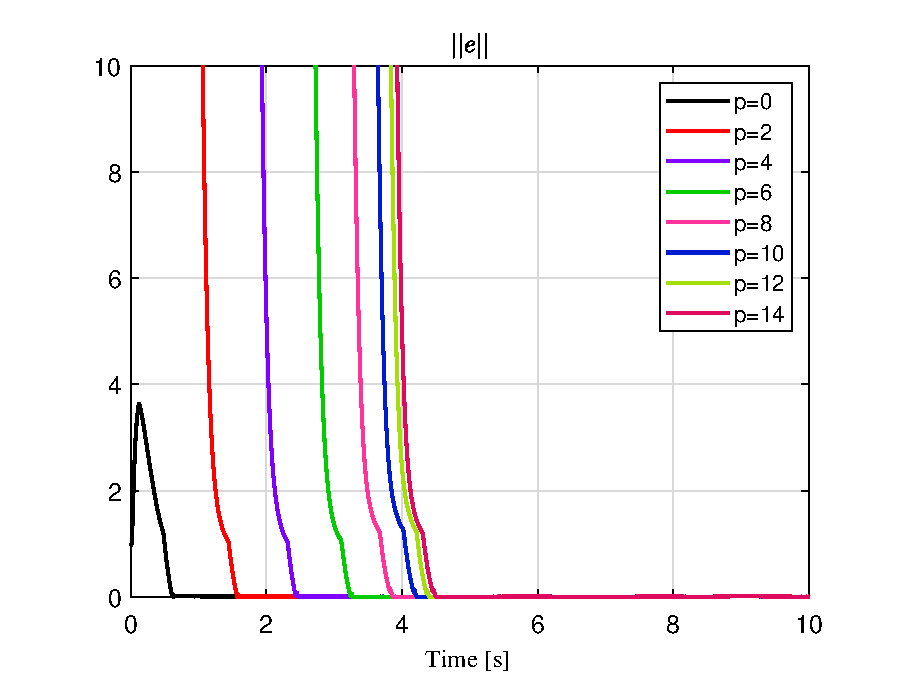
\includegraphics[width=10cm]{sys_4s_disc_FxT_error_orders.eps}}
	\caption{Norm of the estimation error $\norm{e}$ with different orders at initial error. $e_0\times 10^p$.}
	\label{fig: CH4 Error 4s norm with orders}
\end{figure}

\begin{figure}[htbp]
	\centering{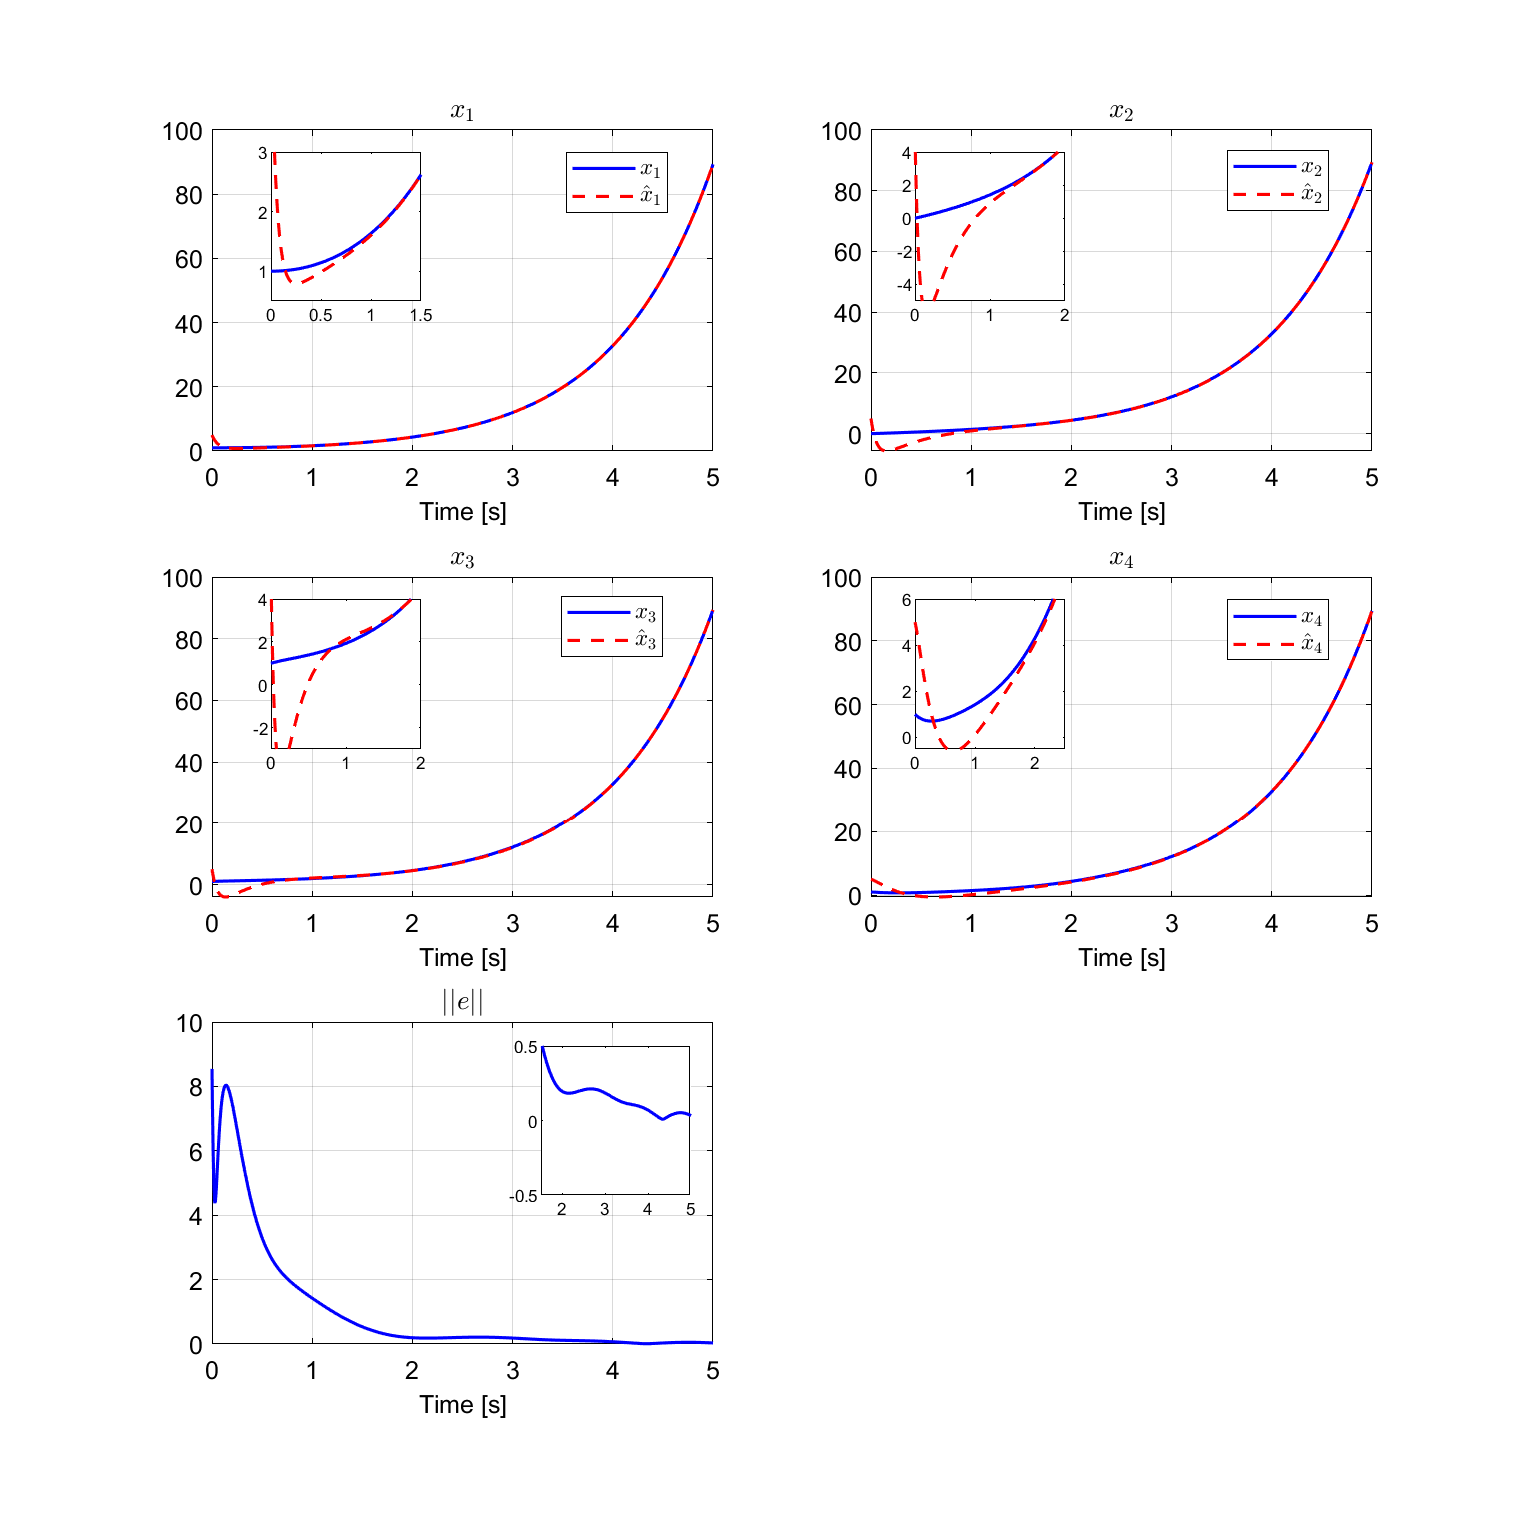
\includegraphics[width=15.8cm]{sys_4s_linear_states.eps}}
	\caption{Estimation of plant states $x_1,...,x_4$ and norm  $\norm{e}$.}
	\label{fig: CH4 Error 4s states and norm, e_0 linear}
\end{figure}

\begin{figure}[htbp]
	\centering{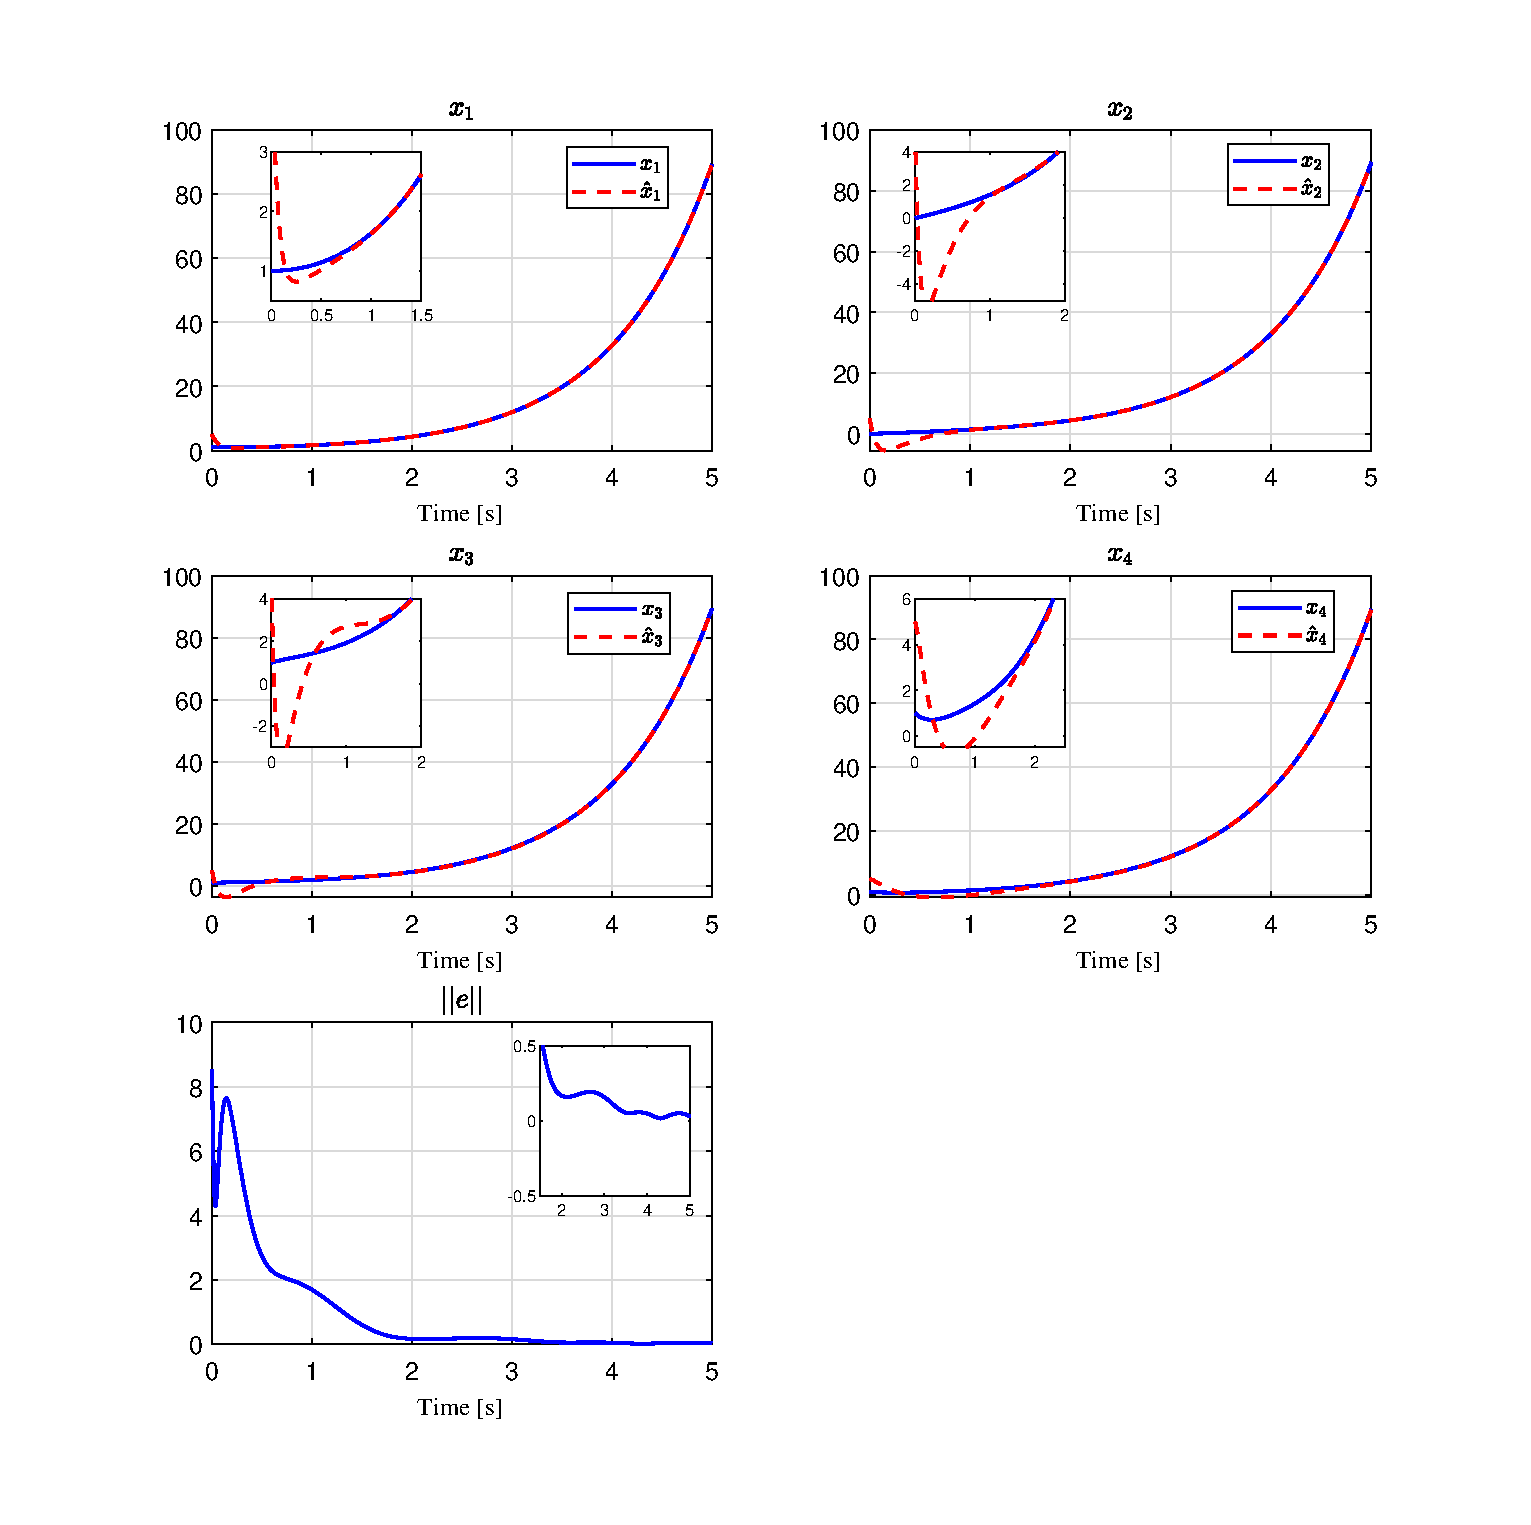
\includegraphics[width=17cm]{sys_4s_cont_states.eps}}
	\caption{Estimation of plant states $x_1,...,x_4$ and norm  $\norm{e}$.}
	\label{fig: CH4 Error 4s states and norm, e_0 cont}
\end{figure}

\begin{figure}[htbp]
	\centering{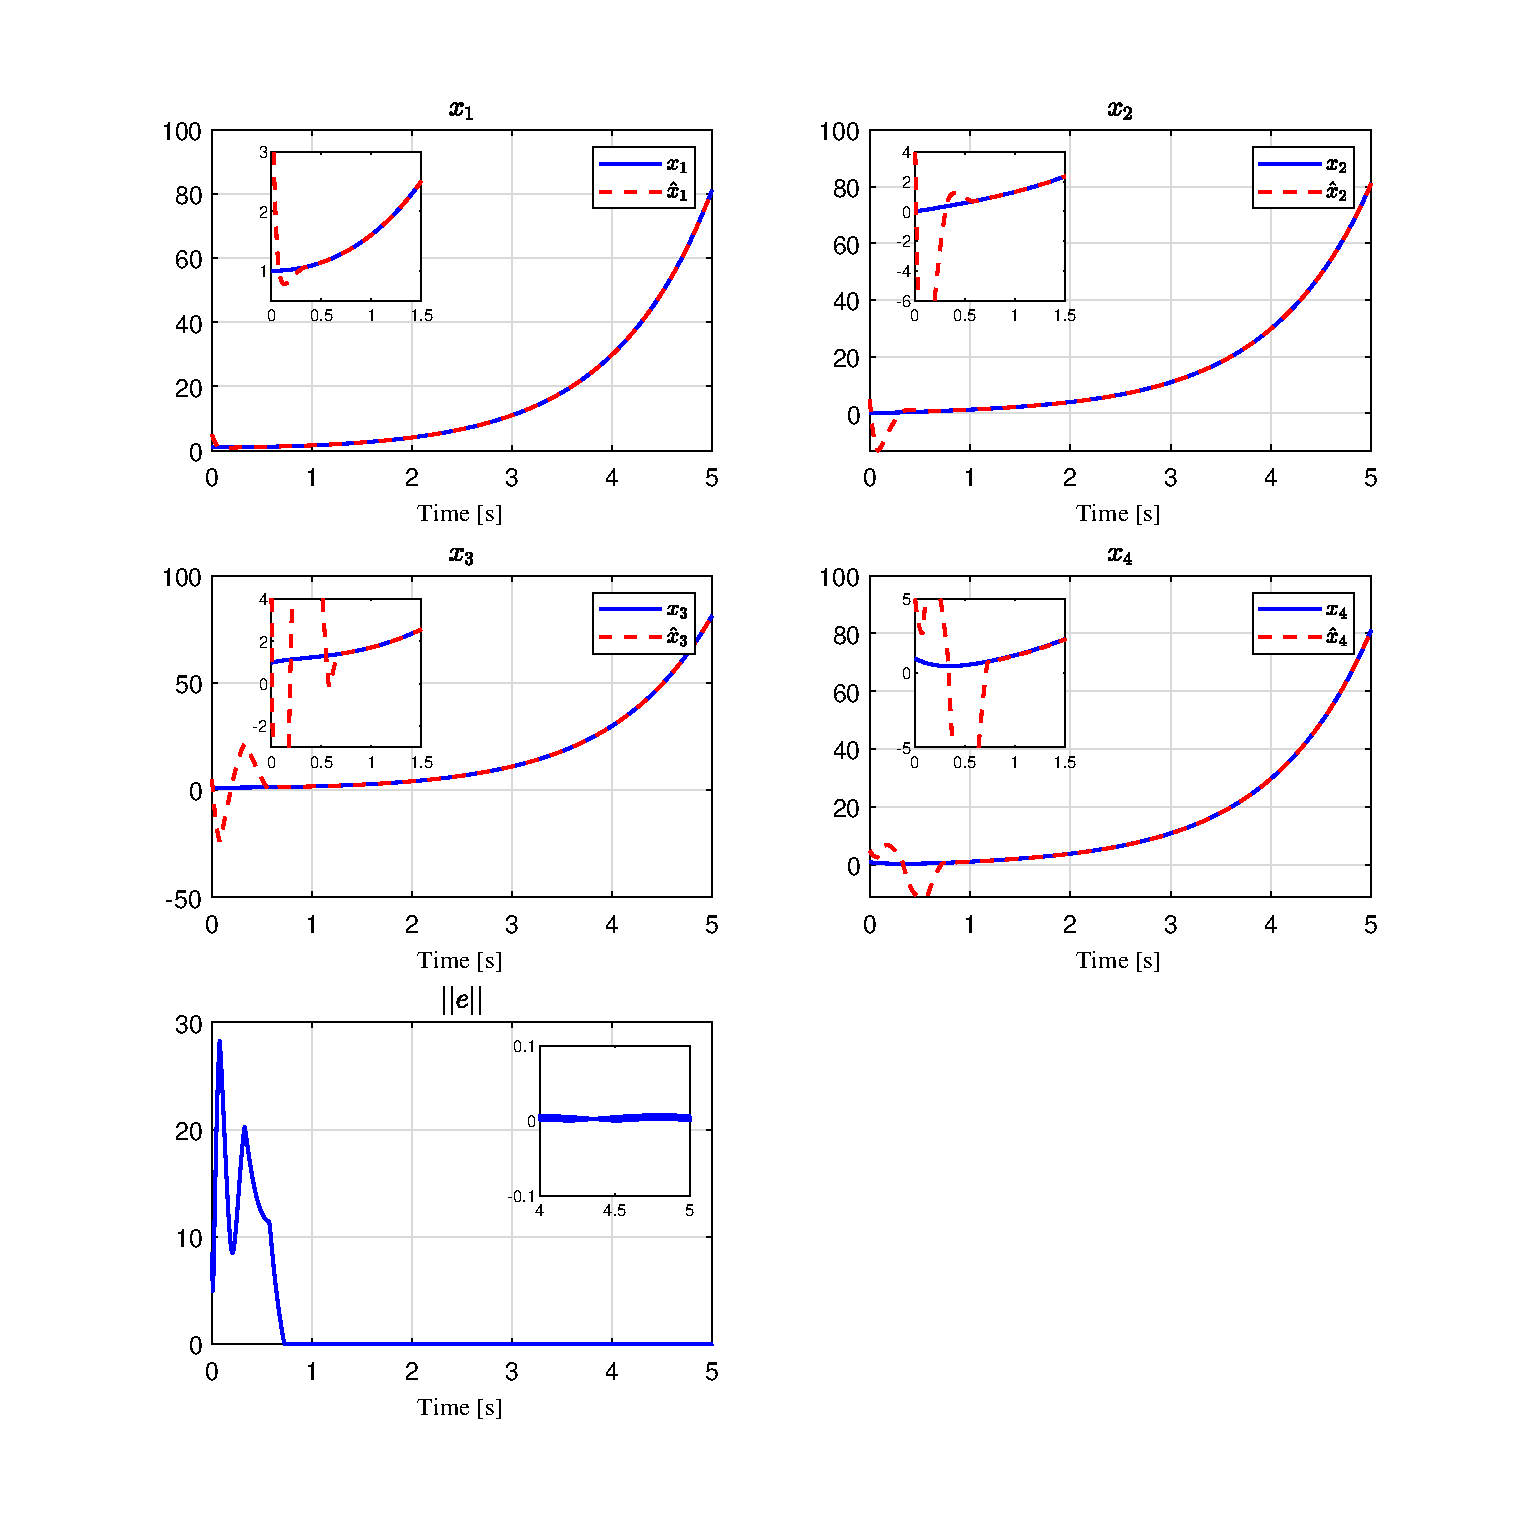
\includegraphics[width=17cm]{sys_4s_disc_states.eps}}
	\caption{Estimation of plant states $x_1,...,x_4$ and norm  $\norm{e}$.}
	\label{fig: CH4 Error 4s states and norm, e_0 disc}
\end{figure}








	%====================================================================
	%                          Bibliografia
	%====================================================================
	\bibliographystyle{ieeetr}
	\bibliography{Citas}
\end{document}